\documentclass{beamer}

\usepackage{beamer_tom}
\graphicspath{{./images/}}
%\usepackage{natbib}

\def\keypoint#1{\hfill\textcolor{gray}{#1}}
\def\mycite#1{\keypoint{\cite{#1}}}
\def\tT{\widetilde{T}}

\institute{\\ INRIA Saclay}
\author{Dupré La Tour T., \textbf{TM}, Mainak J., Gramfort A.}
\title{
	Multivariate Convolutional Sparse Coding for Electromagnetic Brain Signals}

\date{
	May 29, 2018
}

\setbeamertemplate{title page}[frame]
\def\extraLogo{}

\usepackage[titlenumbered,ruled,noend]{algorithm2e}

\begin{document}
	
	\begin{frame}
		\titlepage
	\end{frame}

	\begin{frame}{Studying the brain activty with Electromagnetic brain signal}
	\begin{itemize}
		\item Brain activity produces electromagnetic activity
		\item This can be measured with EEG or MEG
	\end{itemize}

	\begin{columns}[T]
		\column{.5\textwidth}
	\centering
	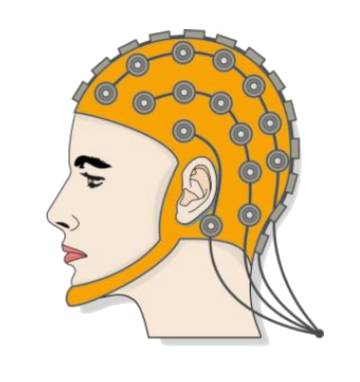
\includegraphics[height=6em]{eeg}\hskip4em
	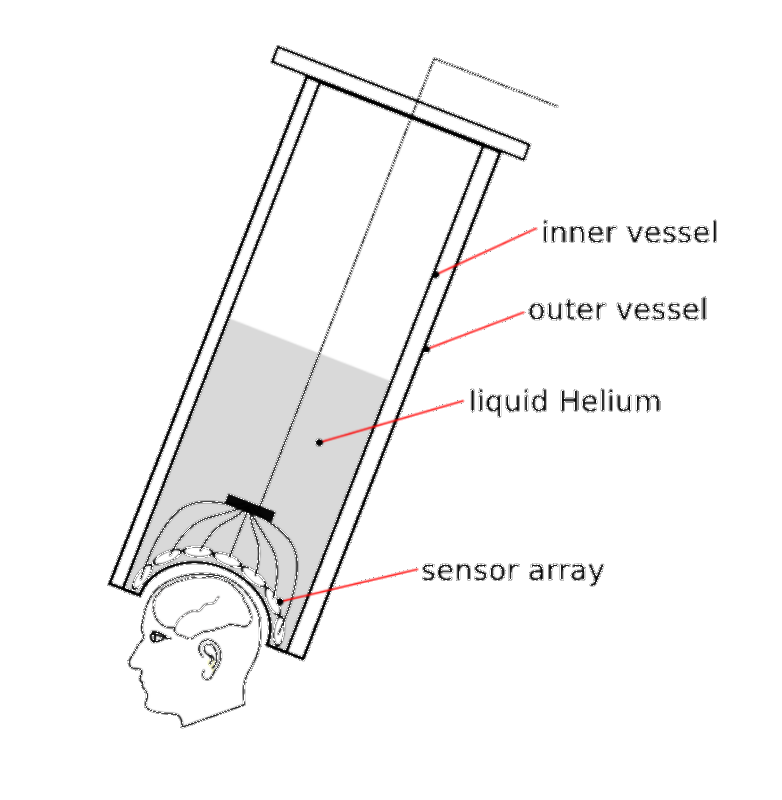
\includegraphics[height=6em]{meg}\\
	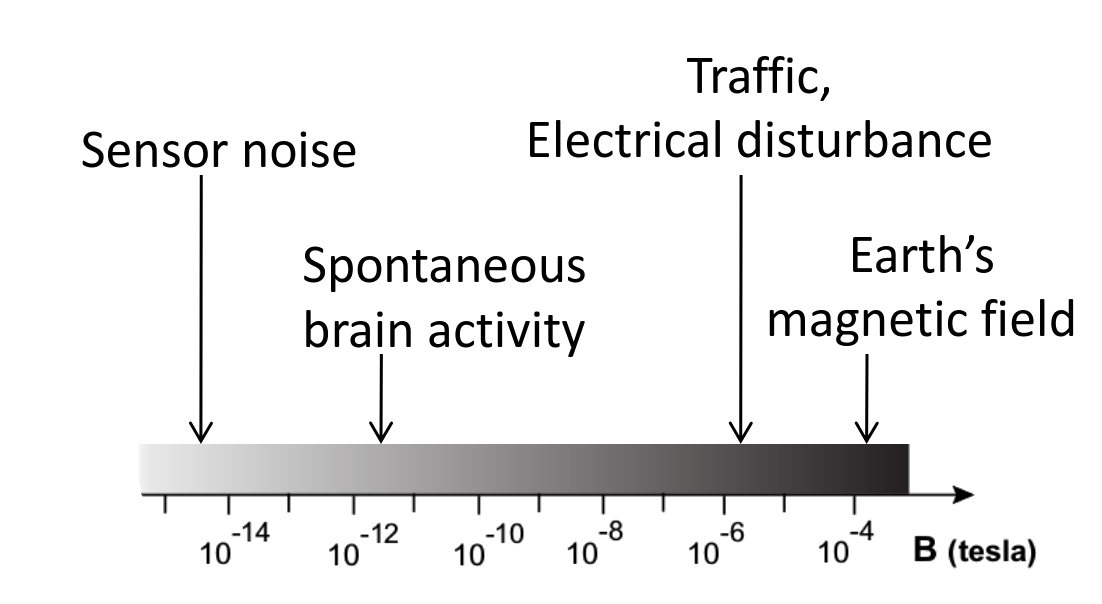
\includegraphics[height=8em]{scale_electro}
	\column{.5\textwidth}
	\vskip3em
	\hskip2em
	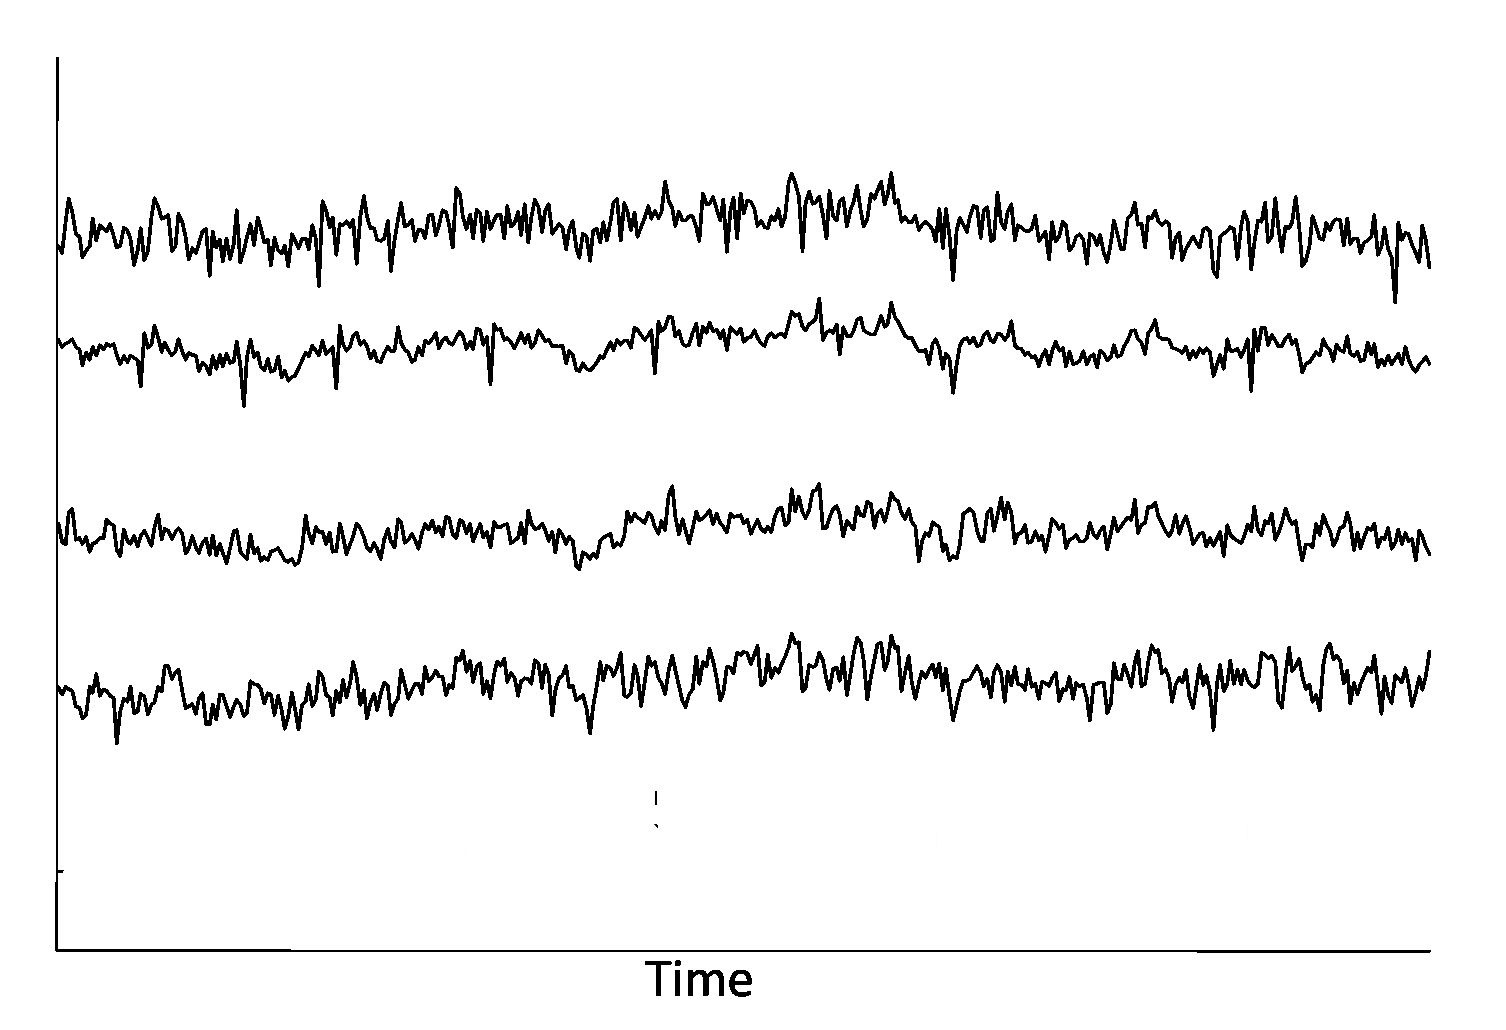
\includegraphics[height=8em]{multivariate_eeg}
	\end{columns}
	\end{frame}
	
	\begin{frame}{%
		Goal: learn representation from neural data}
	
	Many studies rely on Fourier or wavelet analyses, with fixed representation:
	\begin{itemize}
		\item Easy interpretation,
		\item Standard analysis \eg{} canonical bands alpha, beta or theta.\\\mycite{buzsaki2006rhythms}
	\end{itemize}

	\end{frame}

\begin{frame}{Goal: learn representation from neural data}
		However, some brain rhythms are not sinusoidal, \eg mu-waves\mycite{hari2006action}\\
		\hskip5em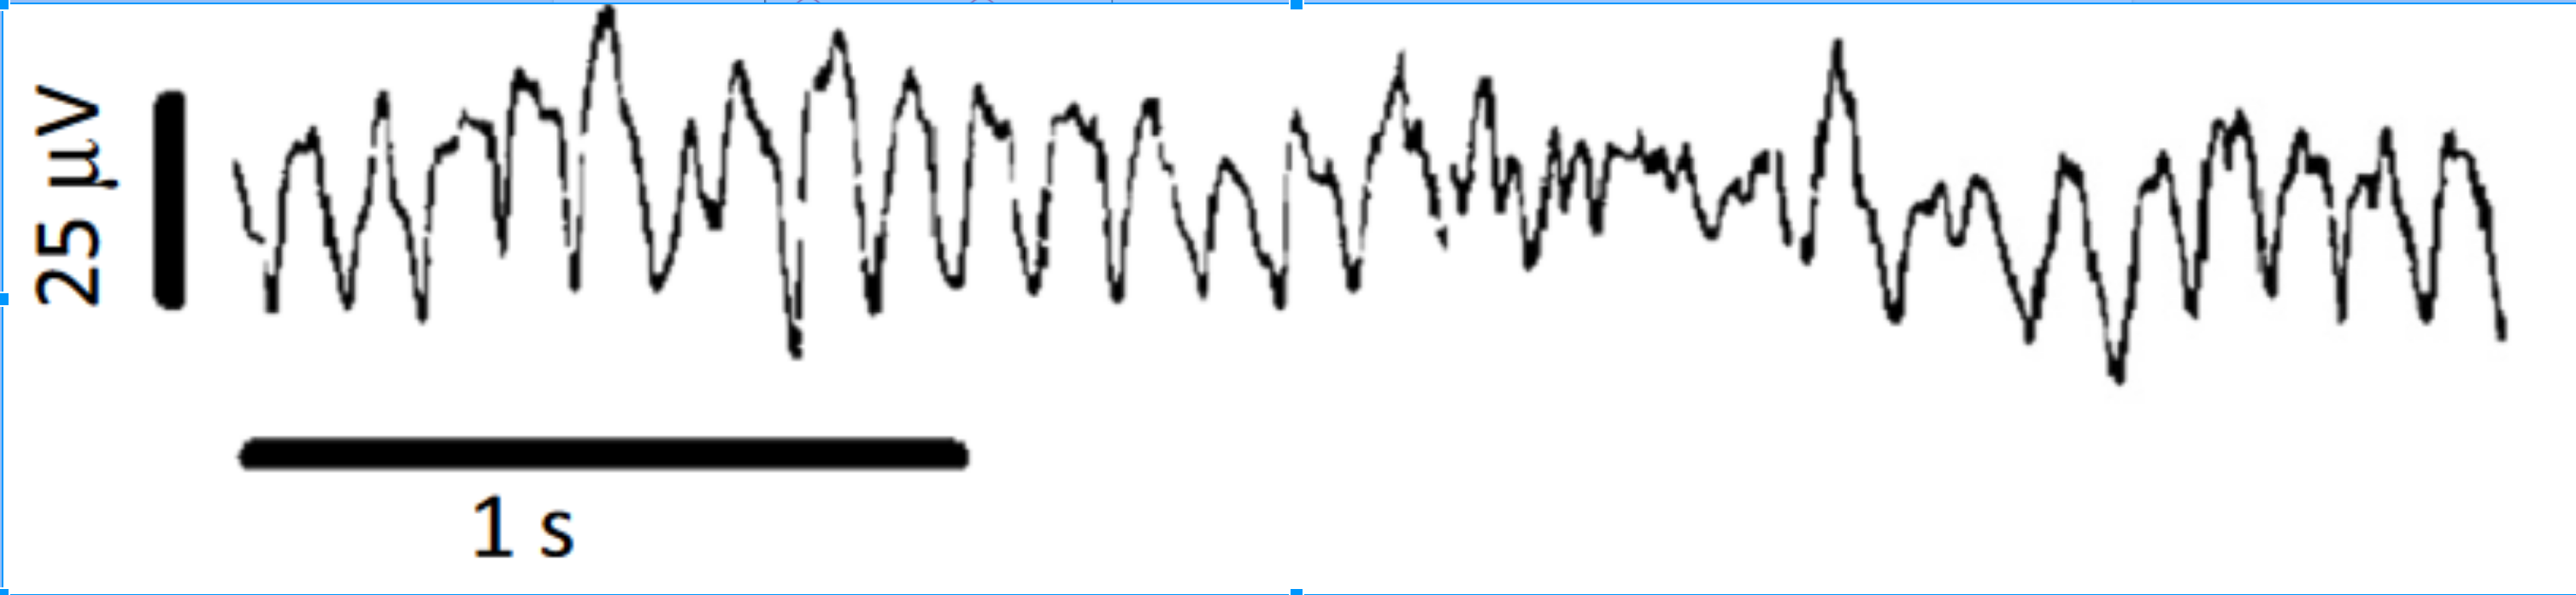
\includegraphics[width=.7\textwidth]{waveform}\\
		and filtering degrades waveforms\\
		\hskip8em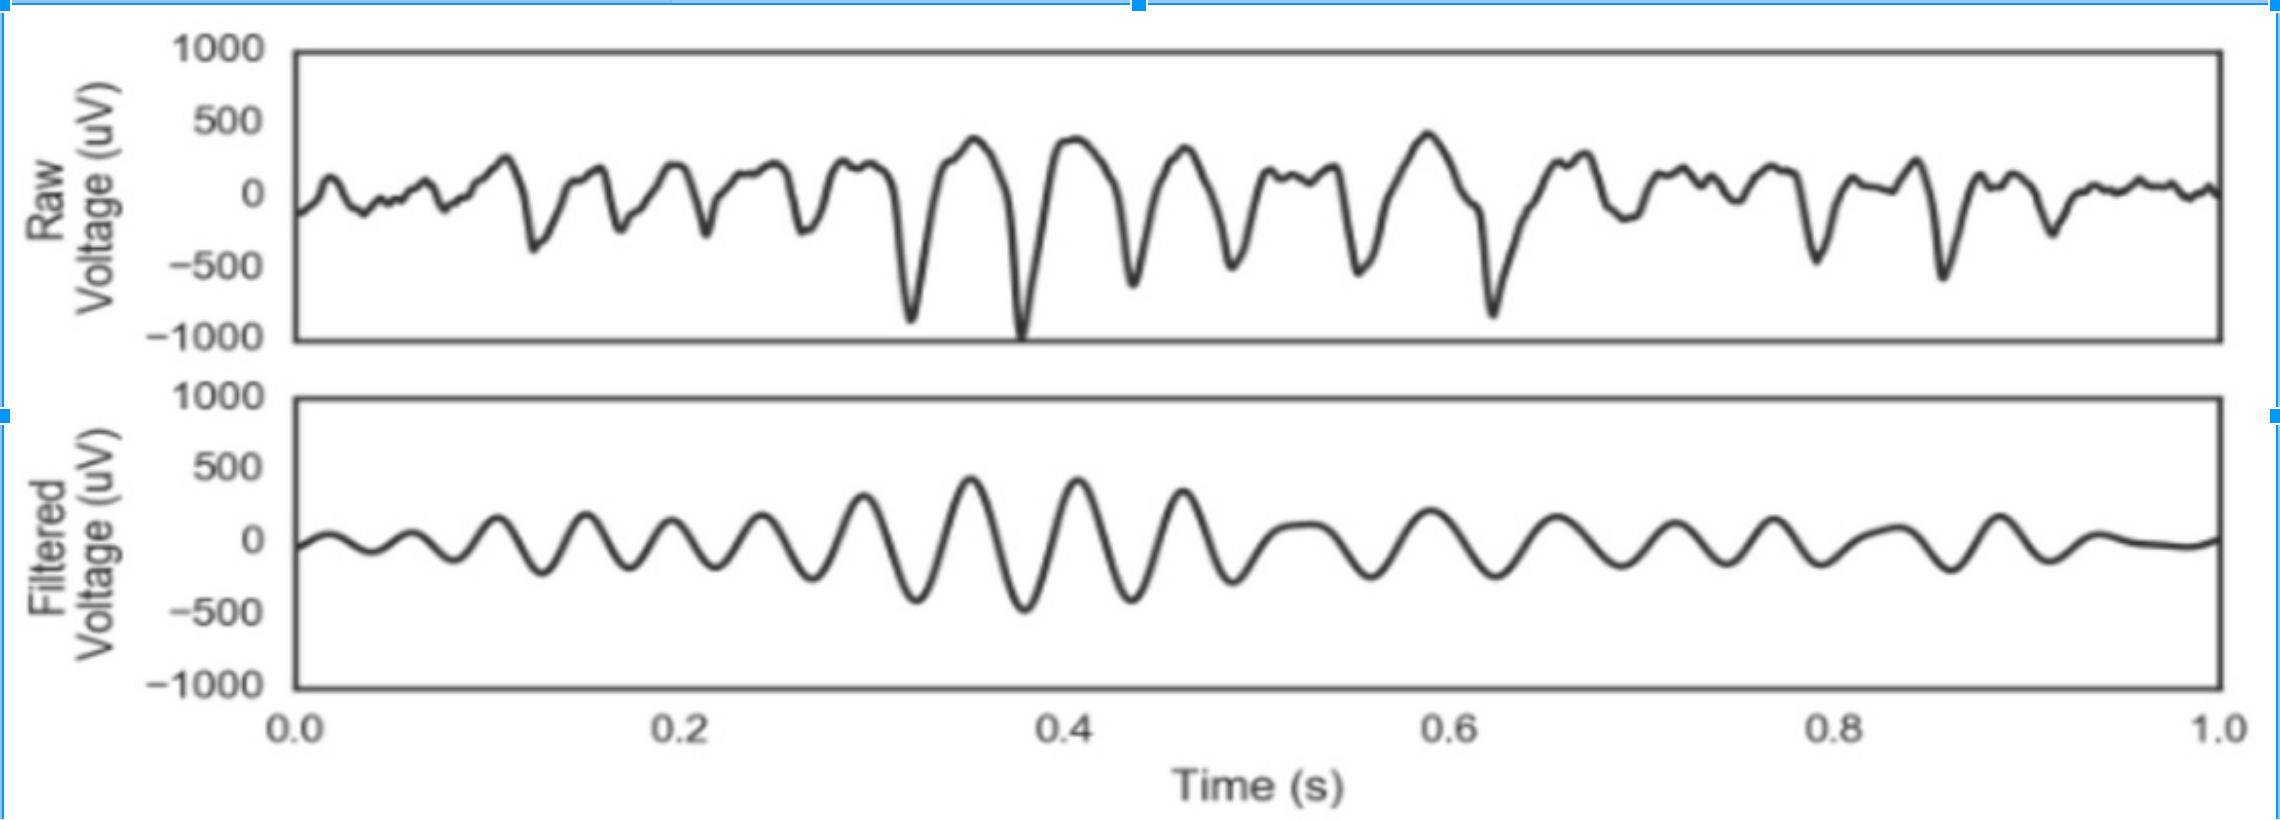
\includegraphics[width=.5\textwidth]{filtering_brain}


	\strongpoint{Can we do better with data-driven approach?}
\end{frame}

\begin{frame}{Extracting shift invariant patterns}
	\textbf{Key idea}: we are not interested in the time-shift of the patterns
	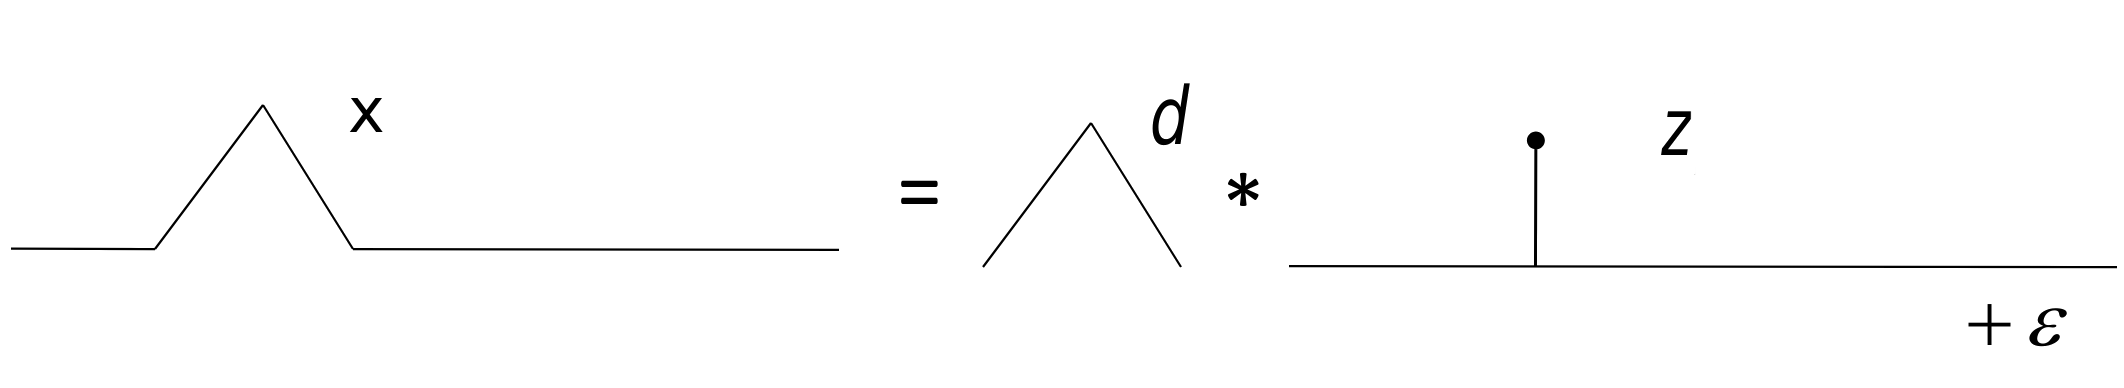
\includegraphics[width=\textwidth]{csc_pattern1}
	\uncover<2->{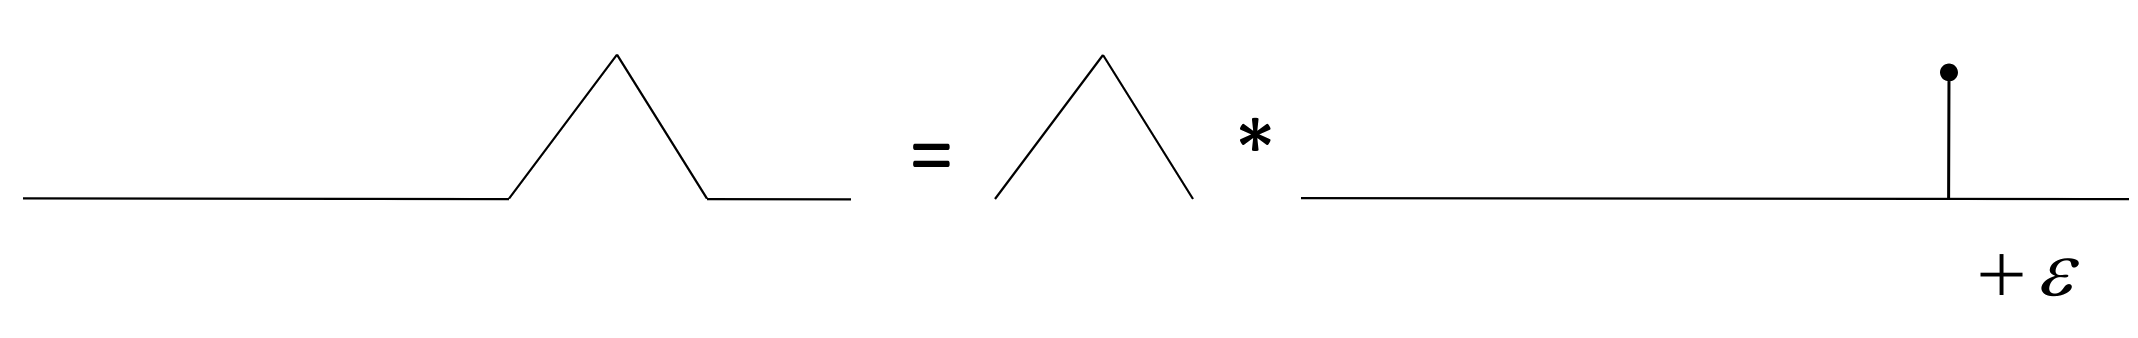
\includegraphics[width=\textwidth]{csc_pattern2}}
	%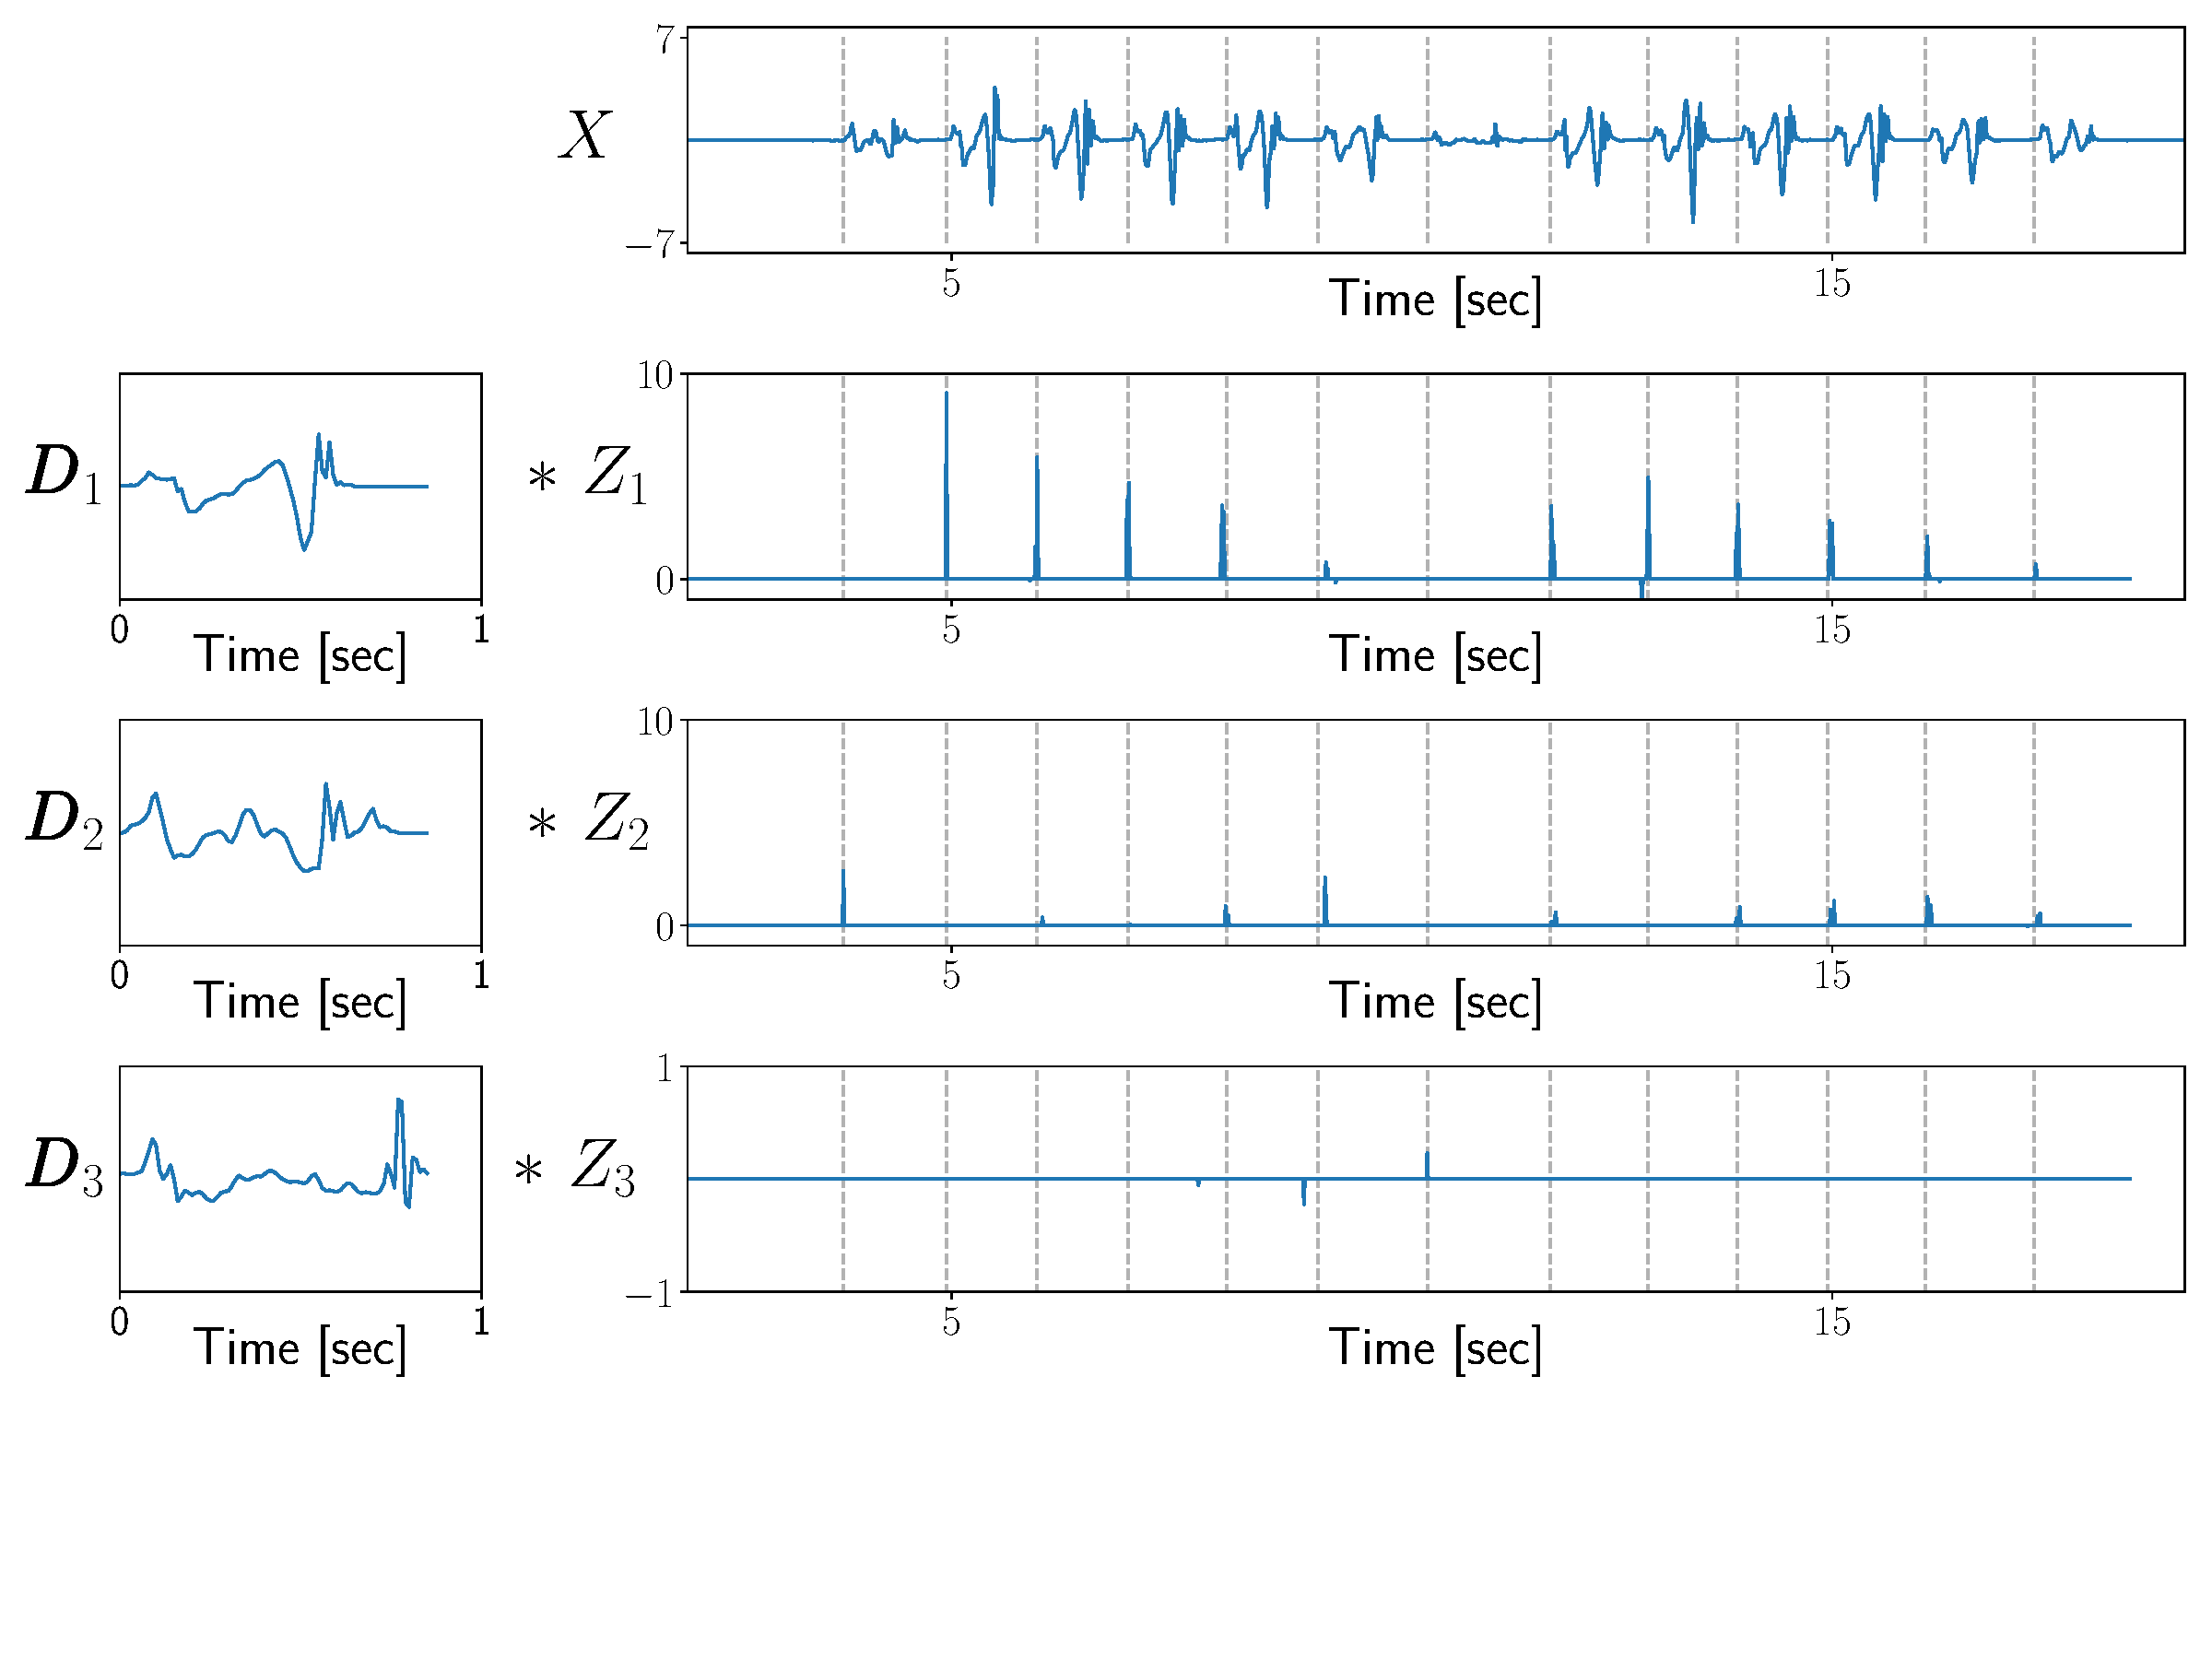
\includegraphics[width=\textwidth]{csc_explain}
	\uncover<3->{Extending this to $K$ patterns:
	\[x = \sum_{k=1}^K d_k * z_k + \mathcal E\]}

	\uncover<4>{\strongpoint{Convolutional representation}}
\end{frame}

\begin{frame}{Convolutional sparse coding}
\textbf{Hypothesis:} patterns are not present everywhere in the signal. They are localized in time.
\strongpoint{Sparse activation signals $z$}
\vskip2em
\textbf{\large Convolutional sparse coding problem (CSC)}\mycite{Grosse2007}\\
For a set of $N$ univariate signals $x^n$, solve
\[
	\min_{d_k, z_k^n} \sum_{n=1}^N\frac{1}{2}\|x^n - \sum_{k=1}^K z_k^n * d_k\|_2^2 + \lambda\sum_{k=1}^K\|z^n_k\|_1
\]
\vskip1em
\textbf{Extra hypothesis:} the activation $z_k^n$ are positive.
\end{frame}

\begin{frame}{How to extend CSC to multivariate signals?}
We can just use multivariate convolution,
\[
	\underbrace{X[t]}_{\in\Rset^P} = \sum_{k=1}^K \left(z_k * D_k\right)[t] = \sum_{k=1}^K \sum_{\tau=1}^L z_k[t-\tau] \underbrace{D_k[\tau]}_{\in \Rset^P}
\]
with:
\begin{itemize}
	\item $X$ a multivariate signal of length $T$ in $\Rset^P$
	\item $D_k$ a multivariate signal of length $L$ in $\Rset^P$
	\item $z_k$ a univariate activation signal of length $\tT = T - L + 1$
\end{itemize}
\vskip1em
However, this model does not account for the physics of the problem.
\end{frame}

\begin{frame}{EM wave diffusion}
	\begin{itemize}
		\uncover<1->{\item Recording here with 8 sensors}
		\uncover<2->{\item EM activity in the brain}
		\uncover<3->{\item The electric field is spread \textbf{linearly} and \textbf{instantaneously} over all sensors (Maxwell equations)}
	\end{itemize}
	\centering
	\only<1>{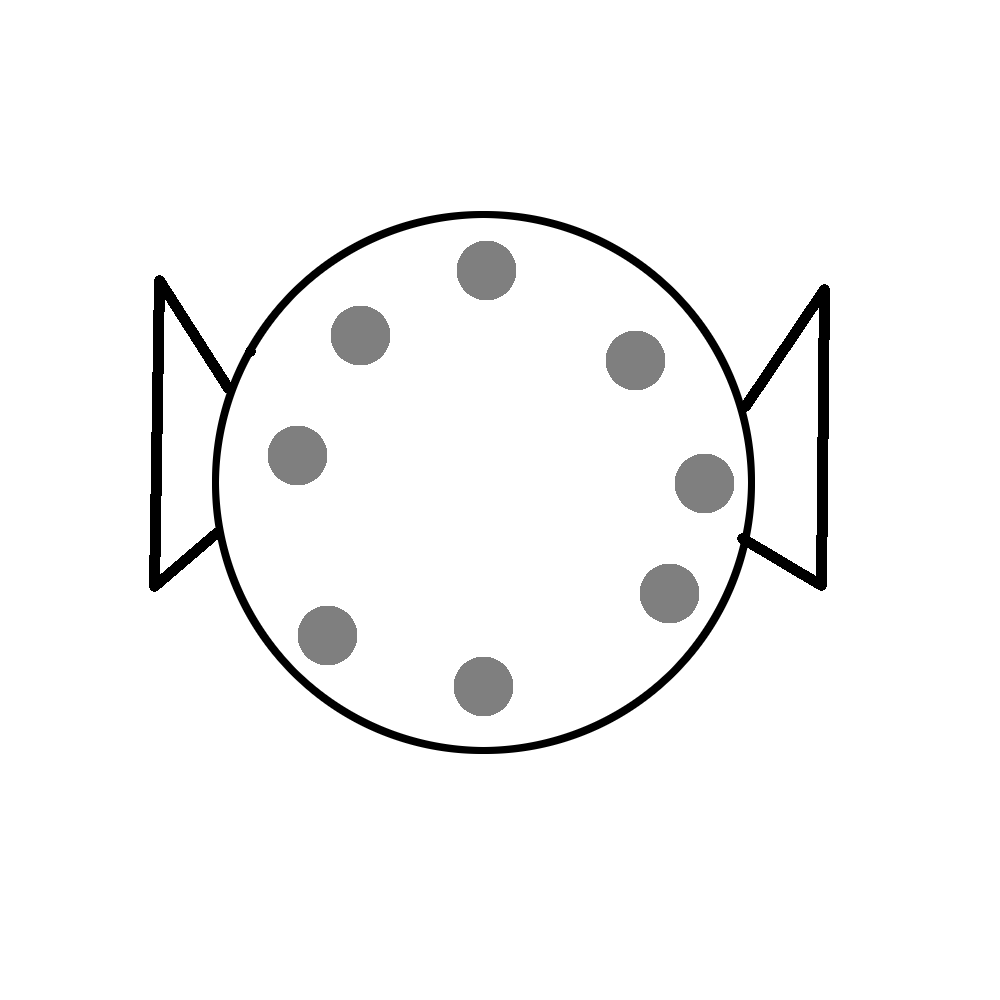
\includegraphics[width=.5\textwidth]{physic1}}%
	\only<2>{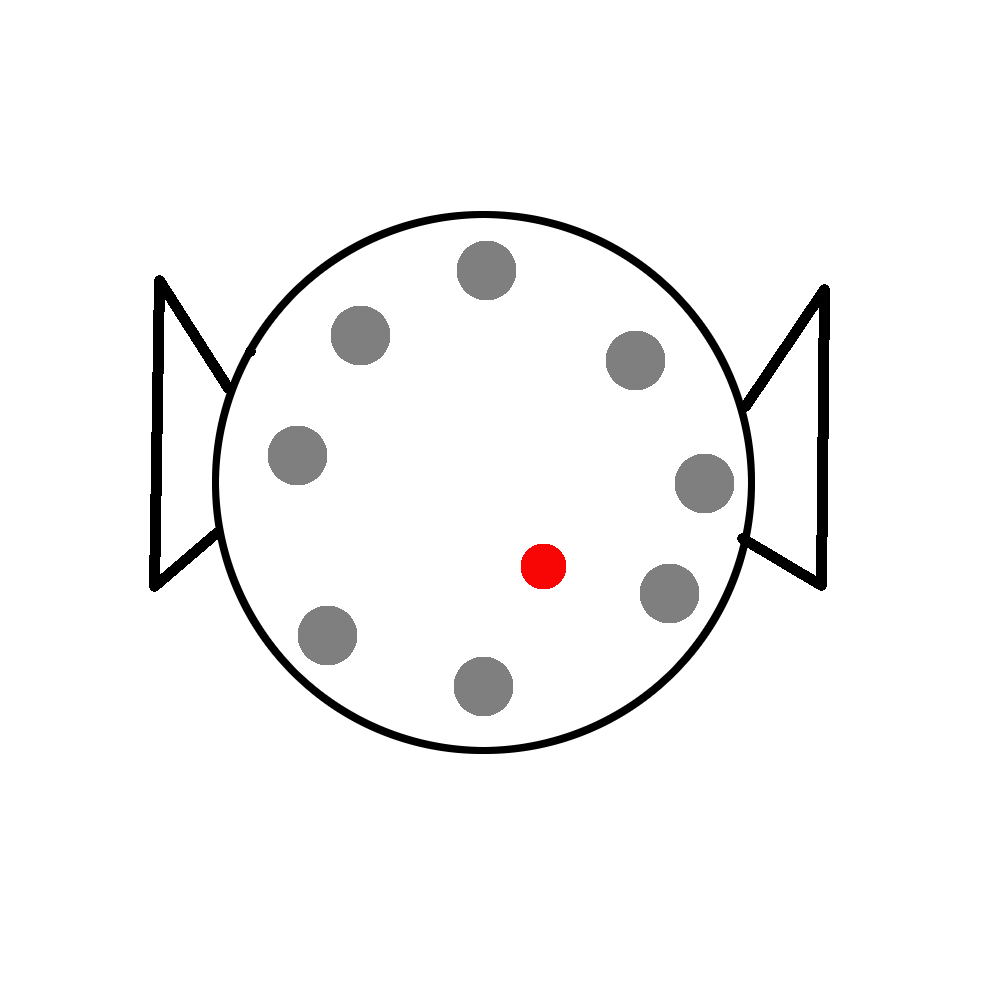
\includegraphics[width=.5\textwidth]{physic2}}%
	\only<3>{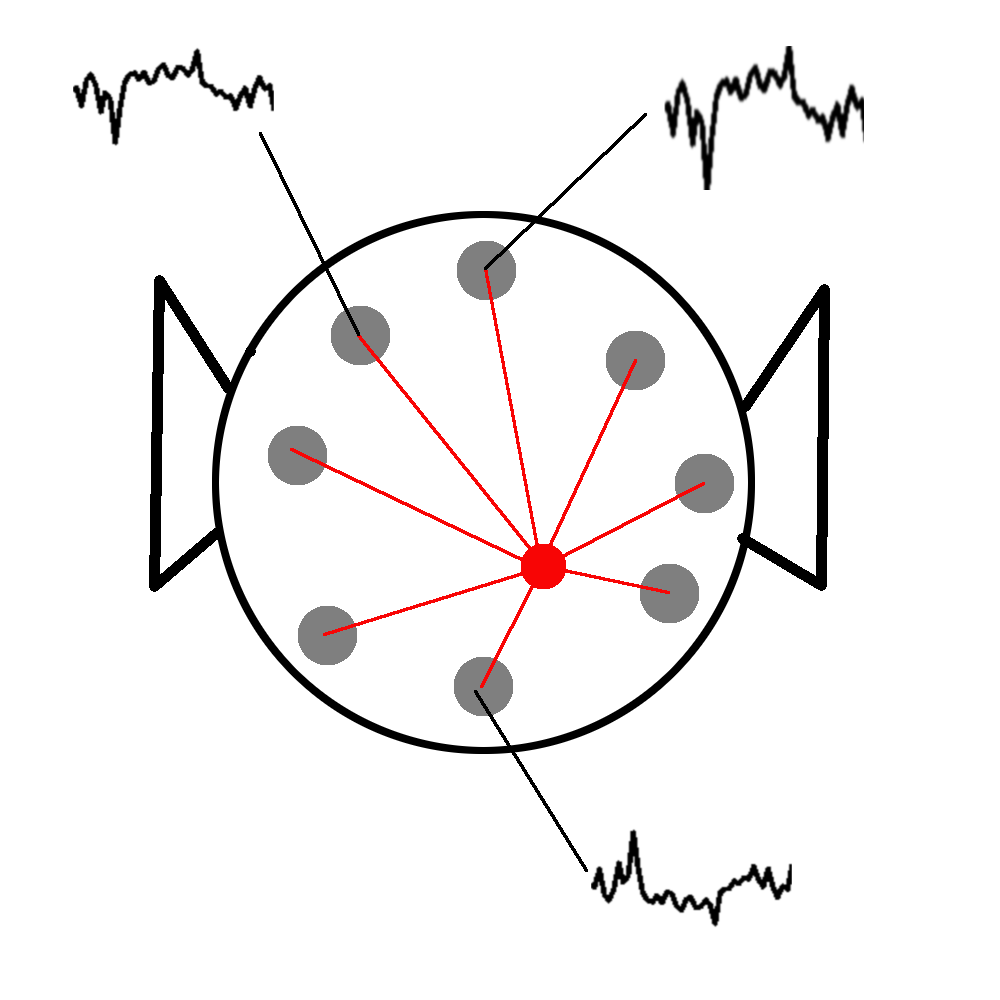
\includegraphics[width=.5\textwidth]{physic3}}
\end{frame}

\begin{frame}{Multivariate CSC with rank-1 constraint}
	\textbf{Idea}: Impose a rank-1 constraint on the dictionary atoms $D_k$
	\vskip1em
	To make the problem tractable, we decided to use auxiliary variables $u_k$ and $v_k$ \st{} $D_k = u_kv_k\top$.
	
	\begin{equation}
	\label{eq:multichannel_csc}
	\begin{split}
	\min_{u_k, v_k, z_k^n} &\sum_{n=1}^N\frac{1}{2}\left\|X^n - \sum_{k=1}^K z^n_k * (u_k^{ } v_k^\top)\right\|_{2}^{2}
	+ \lambda  \sum_{k=1}^K \left\|z^n_k\right\|_1, \hspace{6pt}\\
	&\text{s.t. } ~~ \|u_{k}\|_2^2 \leq 1 \text{  , }\|v_{k}\|_2^2 \leq 1 \text{  and } z_k^n \geq 0~.
	\end{split}
	\end{equation}
	
	Here,
	\begin{itemize}
		\item $u_k \in \Rset^P$ is the spatial pattern of our atom
		\item $v_k \in \Rset^L$ is the temporal pattern of our atom
	\end{itemize}
\end{frame}

\begin{frame}{Optimization strategy}
The problem \autoref{eq:multichannel_csc} is not jointly convex in $z^n_k$, $u_k$ and $v_k$ but it is convex in each block of coordinate.\\[1em]

We can use a block coordinate descent, aka alternate minimization, to converge to a local minima of this problem. The 3 following steps are applied alternatively:

\begin{itemize}
	\item \textbf{Z-step:} given a fixed estimate of the atom, compute the activation signal $z^n_k$ associated to each signal $X^n$.
	\item \textbf{u-step:} given a fixed estimate of the activation and temporal pattern, update the spatial pattern $u_k$.
	\item \textbf{v-step:} given a fixed estimate of the activation and spatial pattern, update the temporal pattern $v_k$.
\end{itemize}
\end{frame}

\begin{frame}{Z-step: Locally greedy coordinate descent (LGCD)}

$N$ independent problem such that
\[
	\label{eq:sparse_code}
	\min_{z_k^n \ge 0} \frac{1}{2} \left\|X^n - \sum_{k=1}^K z_k^n * D_k\right\|_2^2
	+ \lambda\sum_{k=1}^K\left\|z_k^n\right\|_1~.
\]
This problem is convex in $z_k$ and can be solved with different techniques:
\begin{itemize}
	\item Greedy CD \mycite{Kavukcuoglu2013}
	\item Fista \mycite{Chalasani2013}
	\item ADMM \mycite{Bristow2013}
	\item L-BFGS \mycite{Gramfort2017}
\end{itemize}

\strongpoint{These methods can be slow for long signals as the complexity of each iteration is at least linear in the length of the signal.}

\end{frame}

\begin{frame}{Z-step: Locally greedy coordinate descent (LGCD)}
	
	For the Greedy Coordinate Descent, only 1 coordinate is updated at each iteration:
	\mycite{Kavukcuoglu2013}
	\vskip.5em
	\begin{enumerate}
		\item The coordinate $z_{k_0}[t_0]$ is updated to its optimal value $z'_{k_0}[t_0]$ when all other coordinate are fixed:
		\[
				z'_{k}[t] =  \max\left(\frac{\beta_{k}[t] - \lambda}{\| D_{k}\|_2^2}, 0\right) ,
		\]
		with $\beta_{k}[t] = \left[D_{k}^\Lsh * \left(X- \sum_{l=1}^K z_l * D_l +z_{k}[t]e_t* D_{k}\right)\right][t]$
		\item The updated coordinate is chosen greedily by maximizing $|z_k[t] - z'_k[t]|$
	\end{enumerate}

	\vskip.5em
	For each coordinate update, it is possible to maintain the value of $\beta$ with $\mathcal O(KL)$ operations.
	
\end{frame}



\begin{frame}{Z-step: Locally greedy coordinate descent (LGCD)}

	We propose to use the LGCD method proposed in Moreau et al. (2018) which is an extension of GCD.
	With LGCD, the coordinate is instead chosen greedily on one of $M$ contiguous sub-segments of the signal $\mathcal C_m$,
	\[
		\mathcal C_m = \interval{1, K}\times\interval{(m-1)\tT/M, m\tT/M}
	\]
	\vskip1em
	With this strategy, if $M = \lfloor \tT / (2L-1) \rfloor$ the complexity of the coordinate selection and the update of $\beta$ are the same. The overall iteration complexity is $\mathcal O(KL)$ instead of $\mathcal(KT)$.\\[2em]

	If very few coefficients are non-zero in $z_k$, only few iteration are needed and thus this strategy can be very efficient.


\end{frame}



\begin{frame}{Z-step: Locally greedy coordinate descent (LGCD)}

\begin{columns}[T]
	\column{.9\textwidth}
	\begin{algorithm}[H]
		\LinesNotNumbered
		\SetKwInOut{Input}{Input}
		\Input{Signal $X$, atoms $D_k$, number of segments $M$, stopping parameter $\epsilon >  0$, $z_k$ initialization}
		Initialize $\beta_k[t]$\\ % and $z_k[t]$ for all $(k,t)$\\
		\Repeat{$\|z - z'\|_\infty < \epsilon$ }{
			\For{$m = 1$ \KwTo $M$}{
				Compute $z'_{k}[t] =  \max\left(\frac{\beta_{k}[t]-\lambda}{\| D_{k}\|_2^2}, 0\right)$
				for $(k,t) \in \mathcal C_m$ \\
				Choose $\displaystyle(k_0, t_0) = \argmax_{(k, t)\in\mathcal C_m} |z_k[t] - z'_k[t]|$\\
				Update $\beta$\\
				Update the current point estimate $z_{k_0}[t_0]\leftarrow{}z'_{k_0}[t_0]$\\
				%			Set max updates vector $\Delta_m = \left|z_{k_0}[t_0]^{(q+1)} - z'_{k_0}[t_0]\right|$~
			}
			
		}
		\caption{Locally greedy coordinate descent (LGCD)}
		\label{alg:LGCD}
	\end{algorithm}.
\end{columns}

\end{frame}

\begin{frame}{D-step: solving for the atoms}

	We use the projected gradient descent with an Armijo backtracking line-search \cite{Wright1999} for both u-step and v-step for
	\begin{equation}
		\begin{split}
			\min_{\substack{\|u_{k}\|_2 \leq 1\\\|v_{k}\|_2 \leq 1}} E(\{u_k\}_k, \{v_k\}_k) \overset{\Delta}{=} \sum_{n=1}^N\frac{1}{2}\|X^n - \sum_{k=1}^K z^n_k * (u_k^{ }  v_k^\top) \|_{2}^{2} \hspace{6pt}
			\enspace .
		\end{split}
	\end{equation}
	
	One important computation trick is for fast computation of the gradient.
	\[
	\begin{split}
		\nabla_{u_k} E(\{u_k\}_k, \{v_k\}_k) &=  \nabla_{D_k}E(\{u_k\}_k, \{v_k\}_k) v_k ~~ \in \Rset^{P}~,\\
		\nabla_{v_k} E(\{u_k\}_k, \{v_k\}_k) &=  u_k^\top \nabla_{D_k} E(\{u_k\}_k, \{v_k\}_k)  ~~ \in \Rset^L~,
	\end{split}
	\]
	Computing $\nabla_{D_k} E(\{u_k\}_k, \{v_k\}_k)$ can be done efficiently
	\[
	\nabla_{D_{k}} E(\{u_k\}_k, \{v_k\}_k) =  \sum_{n=1}^N (z_k^n)^\Lsh * \left(X^n - \sum_{l=1}^K z^n_l * D_l\right)
	=  \Phi_k - \sum_{l=1}^K \Psi_{k, l} *  D_l \enspace ,
	\]

\end{frame}

\section{Experiments}
\begin{frame}[t]
\vskip5em
\centering
\begin{beamercolorbox}[sep=8pt,center,shadow=true,rounded=true]{title}
	\usebeamerfont{title}\insertsectionhead%
\end{beamercolorbox}
\vskip5em
\flushleft
\large Good time to wake-up if you got lost in the previous section!
\end{frame}

\begin{frame}{Fast optimization}
Comparison with univariate methods on somato dataset with $T=134,700$, $K=8$ and $L=128$\\[1em]
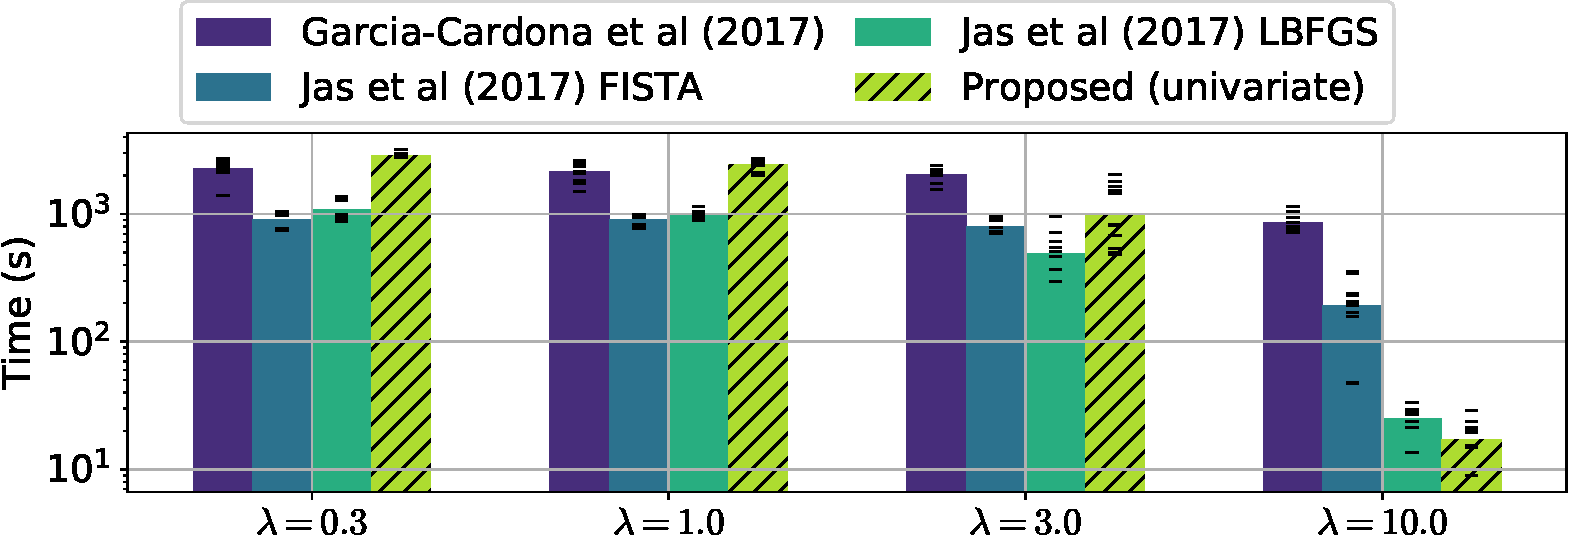
\includegraphics[width=\textwidth]{all_last_0001_T_13470_P1_K8_L128}
\end{frame}

\begin{frame}{Fast optimization}
Comparison with multivariate methods on somato dataset with $T=134,700$, $K=8$, $P=5$ and $L=128$\\[1em]
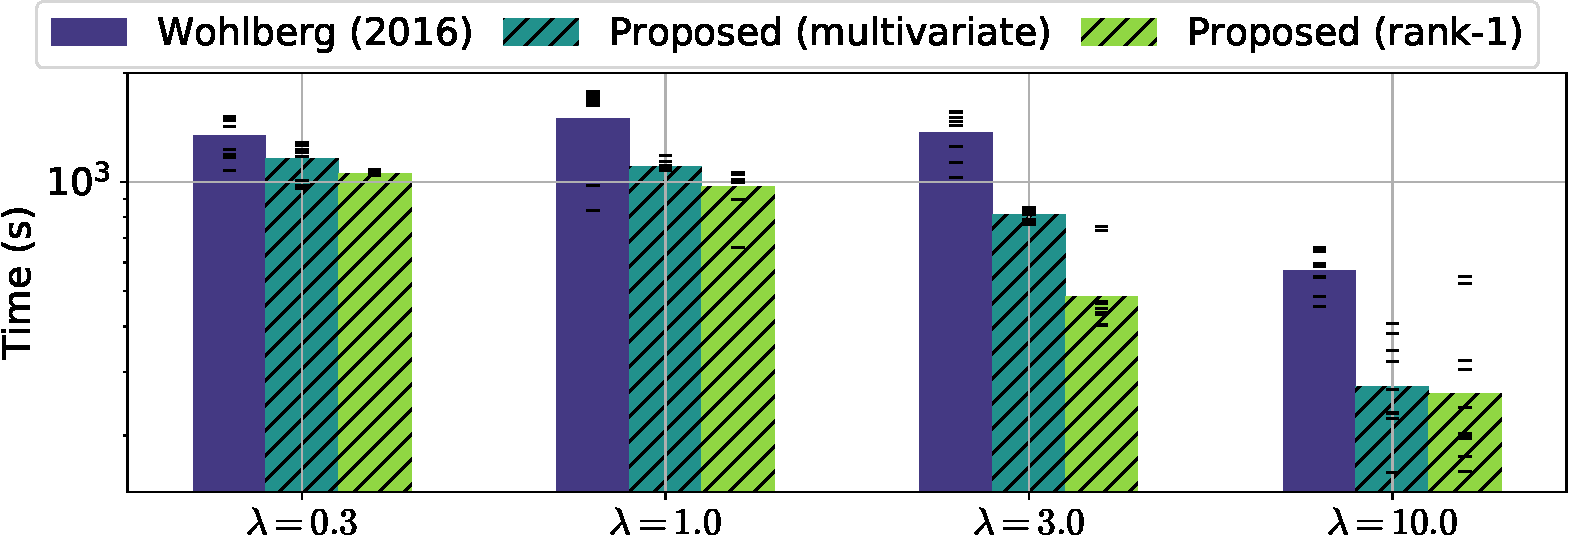
\includegraphics[width=\textwidth]{all_last_0001_T_13470_P5_K8_L128}
\end{frame}

\begin{frame}{Good scaling in the number of channels $P$}
Scaling relative to $P$ on somato dataset with $T=134,700$, $K=2$, and $L=128$\\[1em]
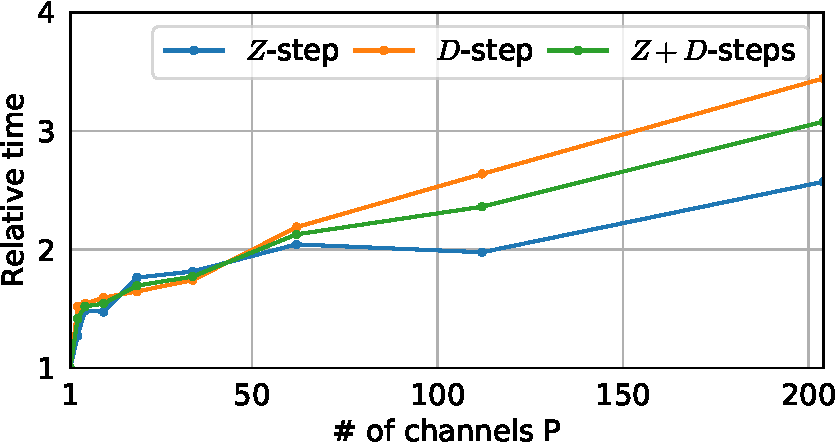
\includegraphics[width=\textwidth]{scaling_channels_reg0_001_mean_rank1_K2_L128.pdf}
\end{frame}

\begin{frame}{Pattern recovery}
Test the pattern recovery capabilities of our method on simulated data,
\[
	X^n = \sum_{k=1}^2 z_k * (u_kv_k^\top) + \mathcal E
\]
where $(u_k, v_k)$ are chosen patterns of rank-1 and the activated coefficient $z^n_k[t]$ are drawn uniformly and their value are uniform in $[0, 1]$.\\[1em]
The noise $\mathcal E$ is generated as a gaussian white noise with variance $\sigma$.\\[1em]

We set $N=100$, $L=64$ and $\tT=640$
\end{frame}

\begin{frame}{Pattern recovery}
Patterns recovered with $P = 1$ and $P=5$. The signals were generated with the two simulated temporal patterns and with  $\sigma = 10^{-3}$. \\[1em]
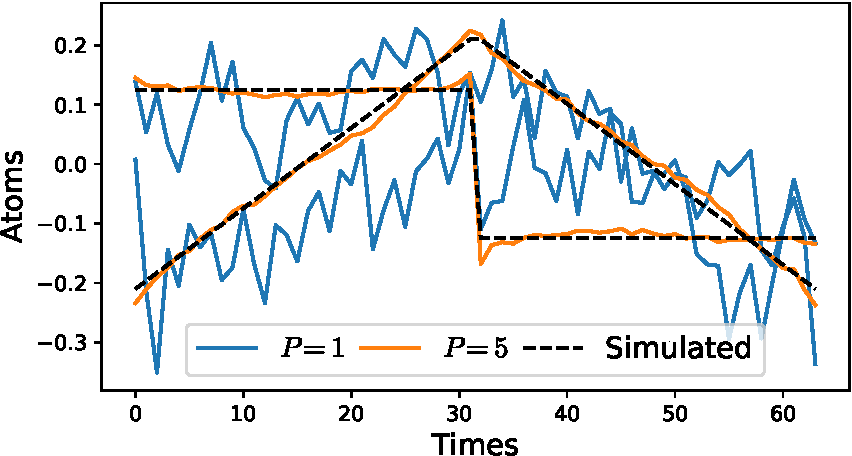
\includegraphics[width=\textwidth]{1D_vs_multi_uv_hat_P5.pdf}
\end{frame}
\begin{frame}{Pattern recovery}
Evolution of the recovery loss with $\sigma$ for different values of $P$. Using more channels improves the recovery of the original patterns.\\[1em]
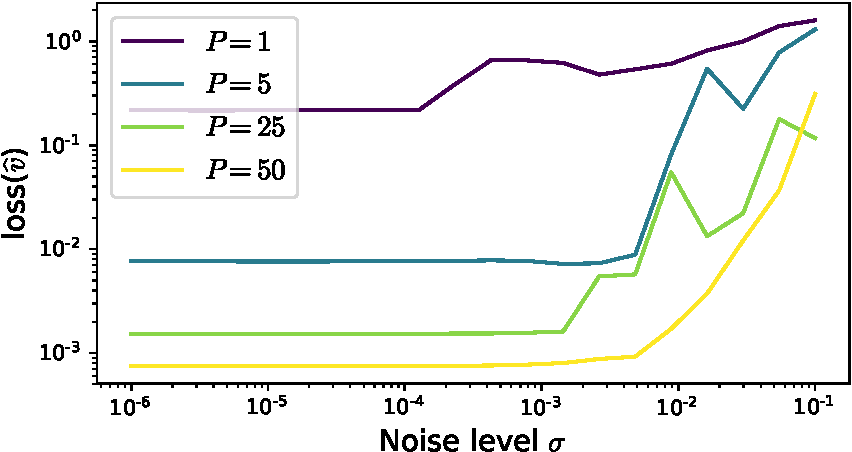
\includegraphics[width=\textwidth]{1D_vs_multi.pdf}
\end{frame}


\section{Experiments on MEG data}
\begin{frame}[t]
\vskip5em
\centering
\begin{beamercolorbox}[sep=8pt,center,shadow=true,rounded=true]{title}
	\usebeamerfont{title}\insertsectionhead%
\end{beamercolorbox}
\vskip5em
\flushleft
\large Even better time to wake-up!
\end{frame}

\begin{frame}{MNE somatosensory data}
A selection of temporal waveforms of the atoms learned on the MNE sample dataset.\\[1em]
\centering
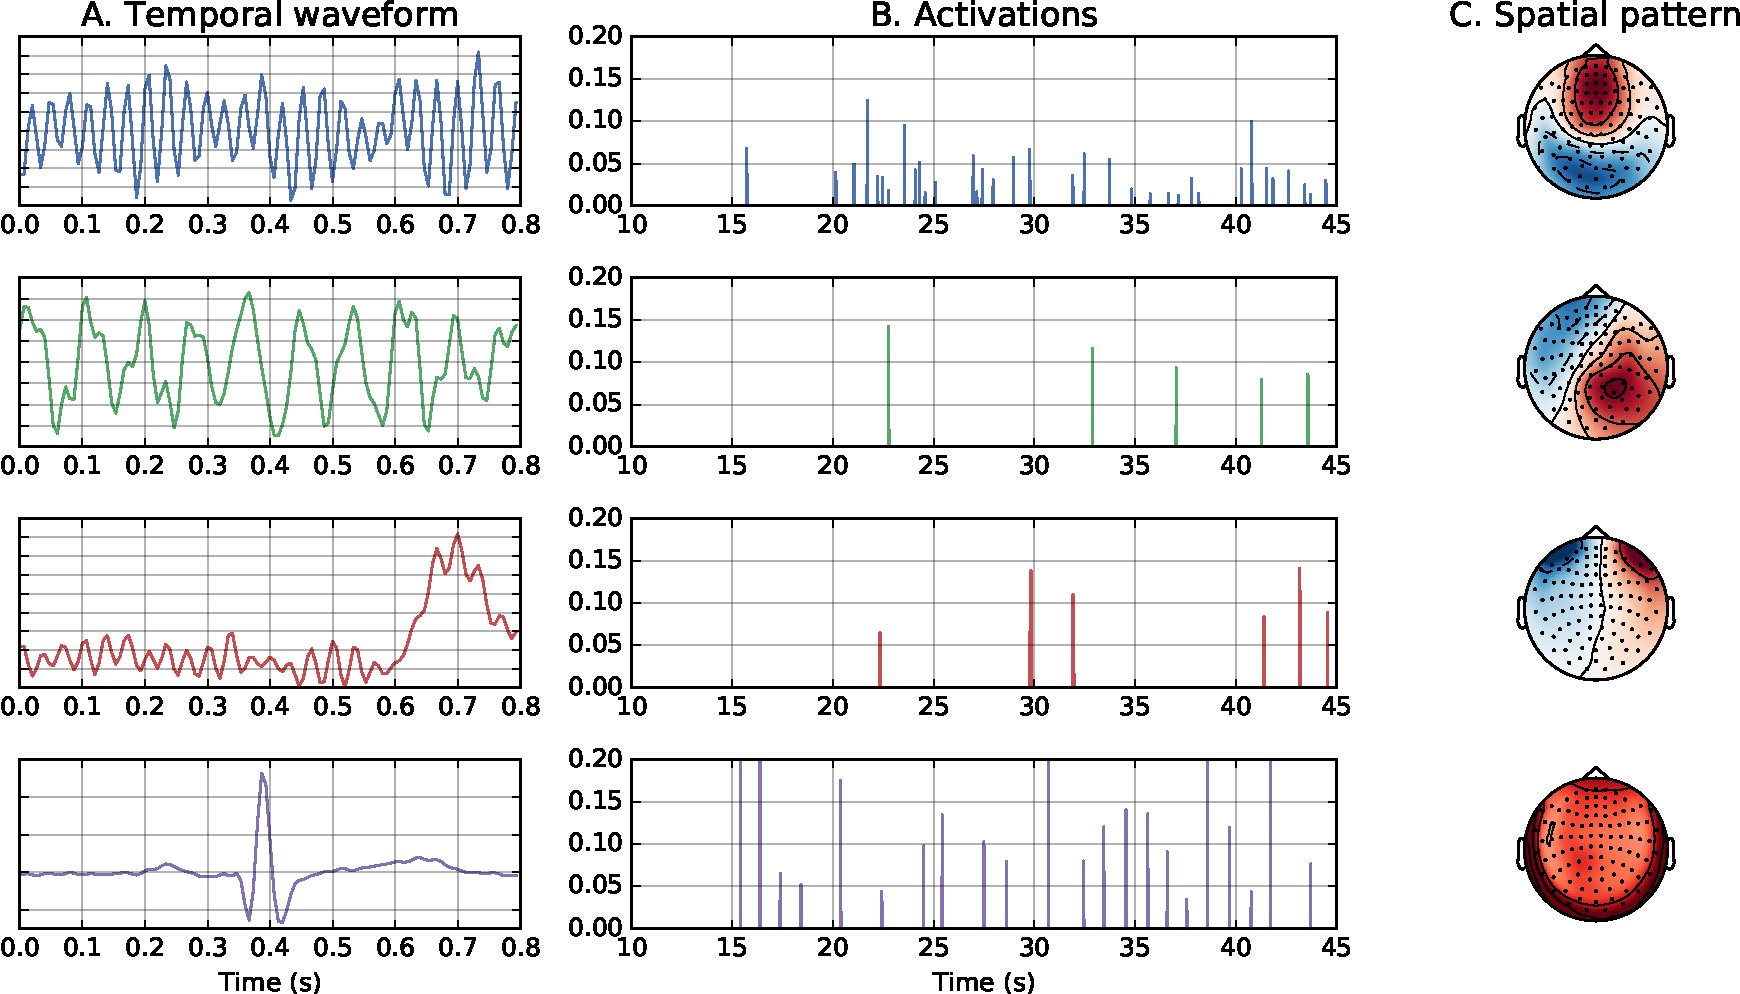
\includegraphics[width=0.99\linewidth]{atoms_sample.pdf}
\end{frame}


\begin{frame}{MNE somatosensory data}
Atoms revealed using the MNE somatosensory data. Note the non-sinusoidal comb shape of the mu rhythm.\\[1em]
\centering
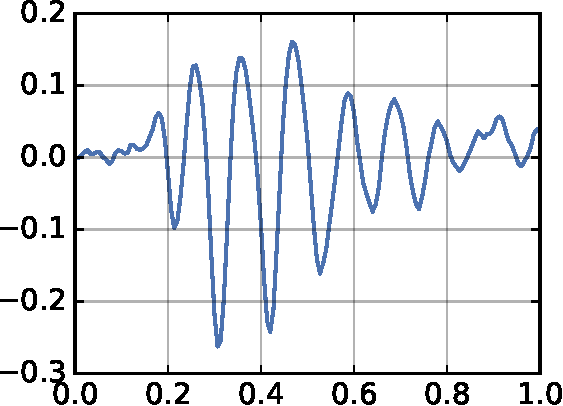
\includegraphics[height=.35\textheight]{atoms_somato_a.pdf}\hskip3em
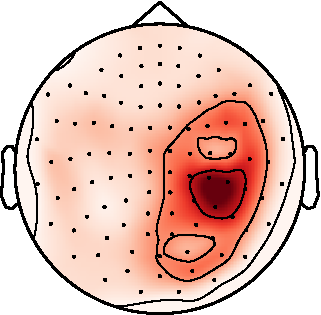
\includegraphics[height=.35\textheight]{atoms_somato_b.pdf}\\[.3em]\hskip1em
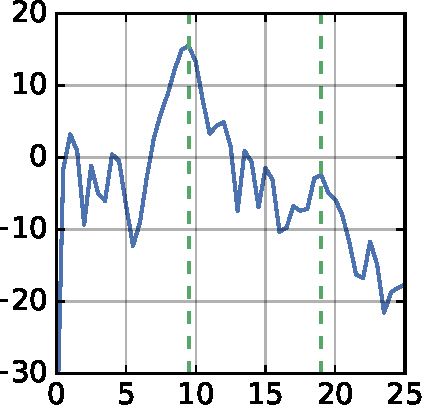
\includegraphics[height=.35\textheight]{atoms_somato_c.pdf}\hskip3em
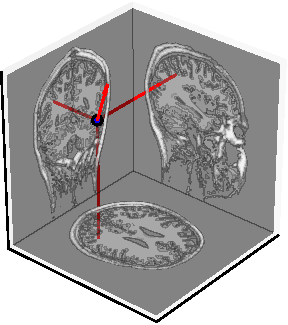
\includegraphics[height=.35\textheight]{atoms_somato_d.pdf}
\end{frame}

\begin{frame}{Conclusion}
	\begin{itemize}\itemsep1.5em
		\item We proposed a model for multivariate CSC with rank-1 constraint. This model makes sense for different type of data.
		\item We proposed a fast algorithm to solve the optimization problem involved in this model.
		\item We demonstrated numerically the performance of our algorithm on both simulated and real datasets.
		\item We illustrated the benefit of such method to study electromagnetic signals form recorded from brain activity. 
	\end{itemize}

\end{frame}

\begin{frame}
\centering
\usebeamercolor[fg]{title}
\usebeamerfont{title}
\Huge \bf Questions?
\end{frame}


\begin{frame}{Reference}
\tiny
\bibliography{library.bib}
\end{frame}
\end{document}
